\section{Lecture 5: Heisenberg Uncertainty}

\subsection{Wave Packet Envelopes}
Consider our thin-in-momentum wave packet from before.

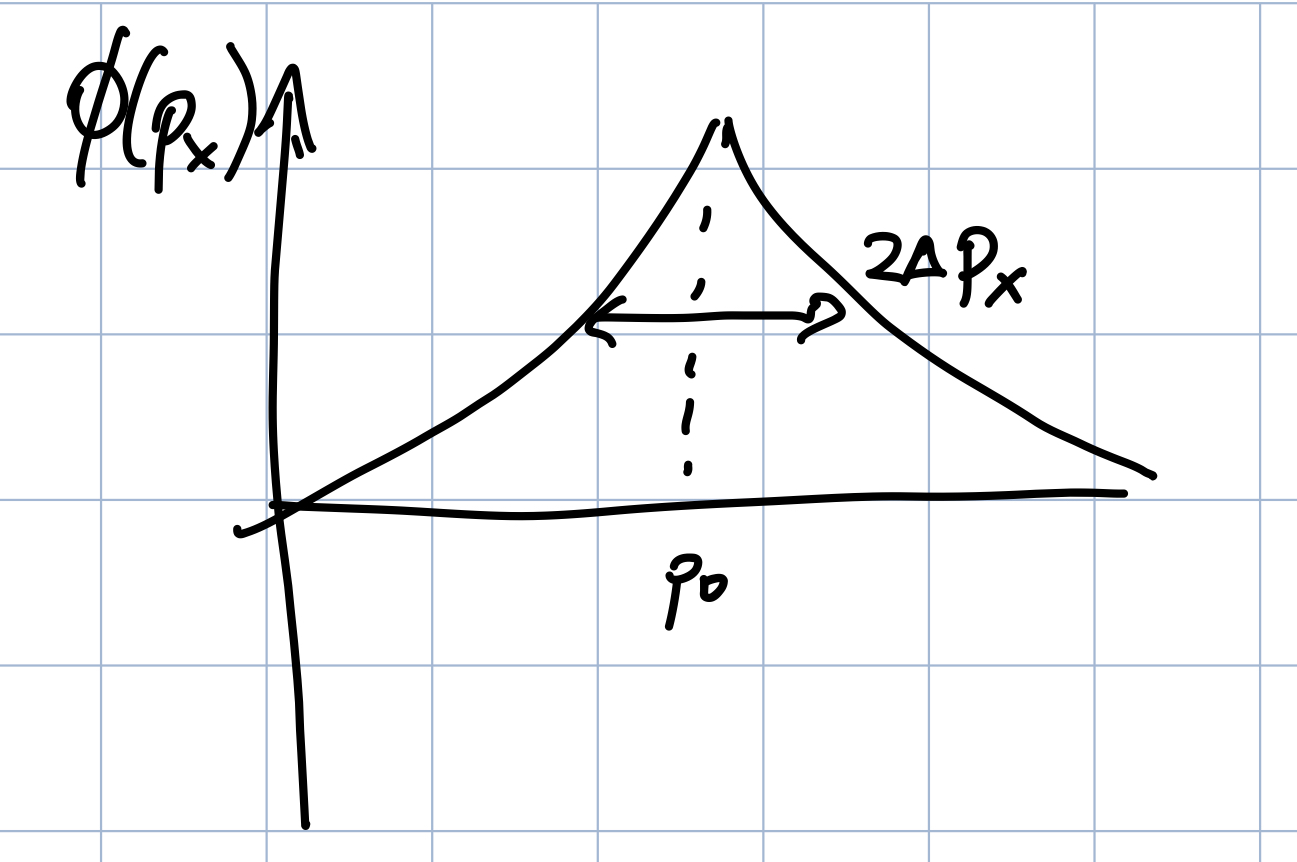
\includegraphics[width=300px]{thin.jpeg}

Recall
\[ v_g = \partialderivative{\omega}{k} \sim \partialderivative{E}{p} \]
Suppose the velocity (for e.g. a point object) is:
\[ v = v_g = \frac{p_x}{m} \]
Then since $v_g$ is $\partialderivative{E}{p}$, the energy can be integrated to be $E = \frac{p_x^2}{2m}$ and we recover the
kinetic energy!

Now we Taylor expand:
\[ E(p_x) = \frac{p_0^2}{2m} + \frac{p_0}{m} (p_x - p_0) + \frac{1}{2m} (p_x - p_0)^2 \]
The first term is $E(p_0)$ and the $\frac{p_0}{m}$ is the group velocity.

So we can write the wavefunction integral:
\[ \Psi(x, t) = \frac{1}{\sqrt{2\pi \hbar}} \int_{-\infty}^{\infty} \exp\qty(i[p_x x - (E(p_0)t + v_gt(p_x - p_0) + \frac{(p_x - p_0)^2}{2m}t)]/\hbar) \phi(p_x) \dd{p_x} \]
We can drop that second order term when:
\[ \frac{(p_x - p_0)^2 t}{2m \hbar} \ll 1 \]
So the wave will disperse (at later time $t$) and spread out! Removing the term yields:
\begin{align*}
    \Psi(x, t) &= \frac{1}{\sqrt{2\pi \hbar}} \int_{-\infty}^{\infty} \exp\qty(i\qty[p_x x - E(p_0)t - v_gt(p_x - p_0)]/\hbar) \phi(p_x) \dd{p_x} \\
    &= \frac{1}{\sqrt{2\pi \hbar}} \int_{-\infty}^{\infty} \exp\qty(i[p_x x - p_0 x + p_0 x - E(p_0)t - v_gt(p_x - p_0)]/\hbar) \phi(p_x) \dd{p_x} \\
    &= \frac{e^{i[p_0 x - E(p_0)t]}}{\sqrt{2\pi \hbar}} \int_{-\infty}^{\infty} \exp(i (p_x - p_0)(x - v_g t)/\hbar) \phi(p_x) \dd{p_x} \\
\end{align*}
The beginning is a plane wave and the integral is a modulating envelope that moves at the group velocity, $v_g$.
Calling
\[F(x, t) = \int_{-\infty}^{\infty} \exp(i (p_x - p_0)(x - v_g t)/\hbar) \phi(p_x) \dd{p_x} \]
The probability density becomes:
\[ |\Psi(x, t)|^2 = |F(x, t)|^2 \]

\subsection{Gaussian Wave Packets}
Now consider the Gaussian wave packet, which in momentum space looks like:



\[ \phi(p_x) = c e^{-(p_x - p_0)^2}{2 (\Delta p_x)^2} \]
Note that $|\phi|^2$ falls to $\frac{1}{e}$ at $p_0 \pm \Delta p_x$. Here is a good Gaussian identity:
\[ \int_{-\infty}^{\infty} e^{-\alpha u^2} e^{-\beta u} \dd{u} = \qty(\frac{\pi}{\alpha})^{1/2} e^{\beta^2/4\alpha} \]
Let us take $\Psi(x) = \Psi(x, 0)$:
\begin{align*}
    \Psi(x) &= \frac{1}{\sqrt{2\pi\hbar}} \int_{-\infty}^{\infty} e^{i p_x x/\hbar} \phi(p_x) \dd{p_x} \\
    &= \frac{1}{\sqrt{2\pi\hbar}} \int_{-\infty}^{\infty} e^{i p_x x/\hbar} \cdot c e^{-(p_x - p_0)^2}{2 (\Delta p_x)^2} \dd{p_x} \\
    &= \frac{\pi^{-\frac{1}{4}} \sqrt{\Delta p_x}}{\sqrt{\hbar}}  e^{i p_0 x / \hbar} e^{-(\Delta p_x)^2 x^2 / 2 \hbar^2}
\end{align*}
Note that the magnitude is a Gaussian. This function falls to $\frac{1}{e}$ of the maximum at $x = \pm \Delta_x$, where
$\Delta x = \frac{\hbar}{\Delta p_x}$. It turns out this is the best you can do.

\begin{theorem}[Heisenberg Uncertainty Principle]
    The Gaussian wave packet is the minimum uncertainty state. That is,
    \[ \Delta p_x \Delta x \geq \hbar \]
    for any wave packet.
\end{theorem}

Furthermore, there is an interplay between frequency and time. Since $E = \hbar \omega$:
\[ \Delta E \delta t \geq \hbar \]

There is a very nice physical interpretation of this principle. If you measure $x$ to an accuracy $\Delta x = a$, then
immediately measuring $p$ would give you an uncertainty at least $\Delta p \geq \frac{\hbar}{\Delta x}$.

\subsection{Heisenberg Microscope}
Suppose you're doing a double-slit experiment and you want to observe what slit the electron went through. We would need to shine some gamma rays
on the electron to look at it. In order for us to measure which slit the electron went to, we definitely need the wavelength to be smaller than the gap between the slits,
$\lambda_{\gamma} < d$. Then:
\begin{align*}
    p_{\gamma} &= \frac{h}{\lambda_{\gamma}} \\
    \Delta p_{e^{-1}} &\sim \frac{h}{\lambda_{\gamma}} \\
    \Delta p_{e^{-1}} &\sim \frac{h}{\lambda_{\gamma}} \geq \frac{h}{d} \\
    d \Delta p_{e^{-1}} &\geq h \\
    \Delta \theta = \frac{\Delta p_{e^{-1}}}{p_{e^{-1}}} &= L \Delta \theta
\end{align*}